% ------------------------------------------------------------------------------
% CHAPTER 4: PAPER 3 (AAS 26-993: EMBEDDED AI ARCHITECTURE)
% ------------------------------------------------------------------------------
\chapter{High-Fidelity Semi-Symplectic Integration under Non-Conservative Forces}
\chaptermark{Semi-Symplectic Strang Splitting}
\label{ch:paper2}

\section*{Chapter Overview and Contextualization}
This chapter addresses the third specific objective of the doctoral research by embedding a multi-tier Artificial Intelligence (AI) architecture directly within the semi-symplectic propagation pipeline. This work synthesizes the methodology and findings published in the \textit{AAS/AIAA Astrodynamics Specialist Conference} (Paper AAS 26-993).

Although the hybrid Strang splitting integrator maintains numerical stability across 50,000 fragments, executing high-density operational tasks---such as pairwise conjunction screening and iterative inverse fragmentation targeting---introduces severe computational latency. Evaluating atmospheric drag using piecewise-exponential lookups introduces gradient discontinuities that perturb the numerical core, while all-on-all conjunction screening scales quadratically ($\mathcal{O}(N^2)$). Furthermore, solving the inverse problem of locating historical breakup coordinates is constrained by file I/O bottlenecks.

To resolve these challenges, this chapter establishes a three-phase AI ecosystem:
\begin{enumerate}
    \item A \textbf{PINN Thermospheric Surrogate} regularized by the differential hydrostatic equilibrium equation to deliver smooth, continuously differentiable density values across LEO.
    \item A \textbf{Spatial KD-Tree} that reduces pairwise distance searches to $\mathcal{O}(N \log N)$, combined with an \textbf{LSTM Sequence Classifier} that accurately identifies high-risk kinematic conjunctions amidst extreme class imbalance.
    \item A \textbf{PPO Reinforcement Learning Agent} connected to the C-compiled symplectic engine via a \texttt{ctypes} shared-memory pointer interface. Operating entirely within hardware RAM across 16 CPU cores, the agent generates 37~FPS, optimizing historical event coordinates without disk serialization overhead.
\end{enumerate}
Computational benchmarks confirm that the integrated AI-symplectic framework preserves the global $\mathcal{O}(N^{1.60})$ power-law scalability curve, providing a scalable computational engine for real-time space traffic coordination.

\newpage
% \includepdf[pages=-, scale=0.95, pagecommand={\thispagestyle{plain}}]{papers/AAS_26_993.pdf}

\clearpage

% Check if the compiled PDF exists; embed if found, display placeholder if missing
\IfFileExists{papers/paper2.pdf}{%
    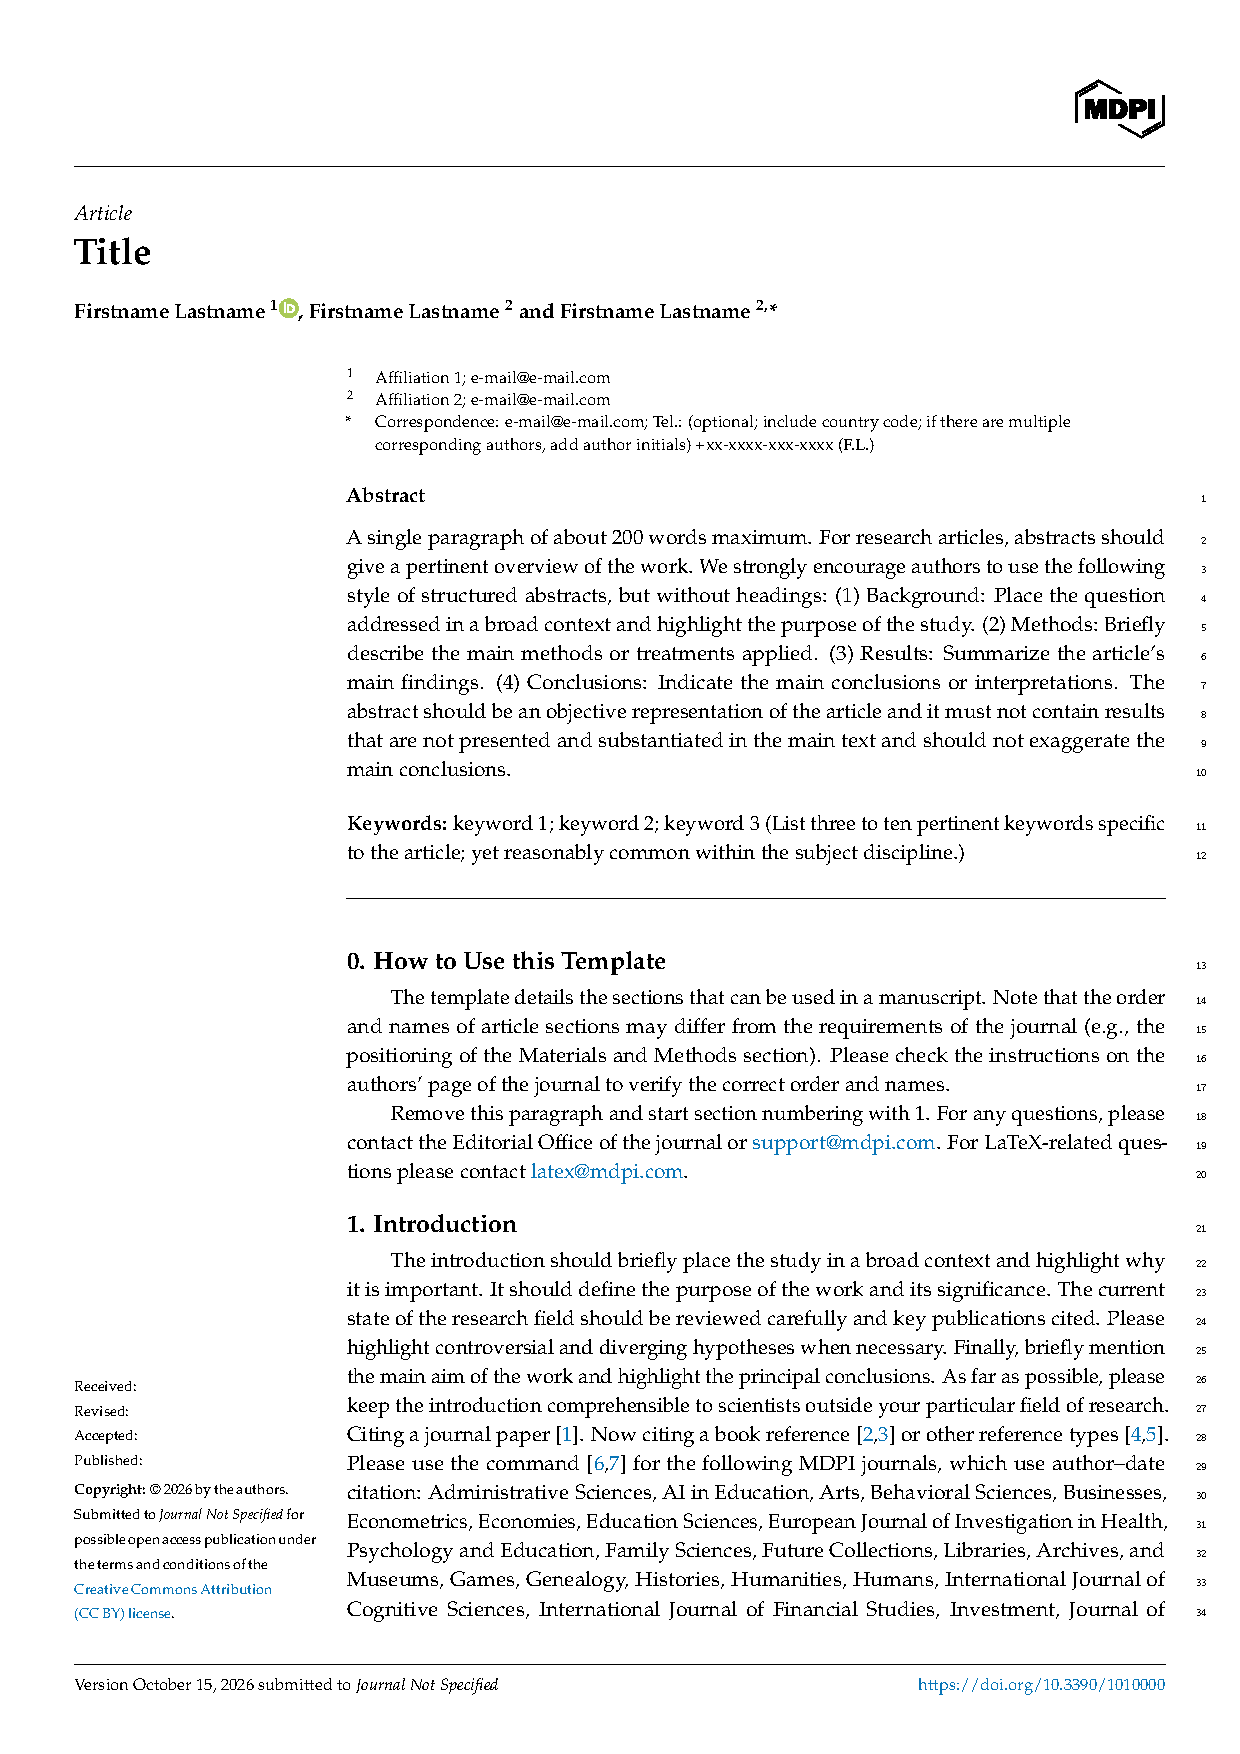
\includepdf[
        pages=-,
        scale=0.95,
        pagecommand={\thispagestyle{plain}}
    ]{papers/paper1.pdf}%
}{%
    \vspace*{2cm}
    \begin{center}
        \fbox{%
            \begin{minipage}{0.85\textwidth}
                \centering\vspace{1cm}
                \textbf{\large [Paper 2 PDF Pending: \texttt{papers/paper2.pdf}]}\\[0.5cm]
                \textit{The compiled PDF was not found in the \texttt{papers/} directory.}\\
                Link or upload the compiled PDF as \texttt{papers/paper2.pdf} to embed the complete publication.
                \vspace{1cm}
            \end{minipage}%
        }
    \end{center}
}